У организаторов всегда возникает проблема в выборе платформы для проведения соревнований.

Основные критерии при выборе платформы:
\begin{itemize}
\item стабильность работы;
\item легкость установки и запуска;
\item наличие примеров работы сервиса.
\end{itemize}

Первые два пункта учитывались на этапе проектирования архитектуры платформы и её разработке, эти пункты описаны в руководстве администратора.
Ниже описаны сервисы, использующиеся как пример работы сервиса и позволяющие глубже понять логику работы платформы.

\subsection{Сервис whoami}
При разработке сервиса было поставлено несколько целей:
\begin{itemize} 
\item Тестирование программного комплекса;
\item Проведение тренировочной игры для команды;
\item Упаковка сервиса в <<стартовый набор>> для ознакомления.
\end{itemize}

Сервис писался на языке Python с использованием базы данных MongoDB и микрофреймворка Flask.

Тестирование платформы заключалось в тестировании следующий функций:
\begin{itemize} 
\item Работа чекера (методы check, get, put);
\item Работа модуля сдачи флагов;
\item Работа платформы в условиях медленного <<ответа>> сервиса.
\end{itemize}

Смысл сервиса состоит в том, что при регистрации пользователь указывает свою электронную почту, пароль и имя.
Если пользователь уже регистрировался, то он просто входит в систему, при условии, что логин и пароль  совпадают. Далее пользователь видит приветственное сообщение в формате <<Привет, <имя пользователя>>>

\begin{figure}[ht!]
\center{
\includegraphics[width=0.5\linewidth]{eco/images/dima_main.png}}
\caption{Главная страница сервиса}
\end{figure} 

Несмотря на простоту сервиса, в нем содержится несколько уязвимостей:
\begin{itemize} 
\item Открытый порт БД (незащищенный паролем);
\item Уязвимость в данных cookie;
\end{itemize}



\subsection{Сервис blozhik}
Сервис был написан для:
\begin{itemize} 
\item проверки корректности работы платформы;
\item выявление возможных проблем, которые могут произойти на соревнованиях;
\item проведения тренировочной игры.
\end{itemize}

Сервис писался на языке Python с использованием микрофреймворка Flask.

Тестирование платформы заключалось в тестировании следующий функций:
\begin{itemize} 
\item Работа чекера (методы check, get, put);
\item Работа модуля сдачи флагов.
\end{itemize}

Смысл сервиса состоит в том, что в веб-приложении существует возможность добавления и удаления "to do" записей (задачи для выполнения). Также есть функции регистрации и авторизации, т.е. каждый пользователь видит только свои "to do".

Сервис содержит несколько уязвимостей:
\begin{itemize} 
\item backdoor, с проверкой cookies;
\item внедрение SQL кода в cookies (' OR '1'='1);
\item внедрение SQL запроса в записи "to do" (подмена владельца записи "to do").
\end{itemize}

Ниже приведен скриншот работы сервиса (Рисунок 7.2).
\begin{figure}[ht!]
\center{
\includegraphics[width=0.8\linewidth]{eco/images/timur_t.png}}
\caption{Сервис todolist}
\end{figure}

\subsection{Zabbix}
В нашем проекте Zabbix был использован для: 
\begin{itemize} 
\item мониторинга состояния сети; 
\item контролирование ресурсов сервера.
\end{itemize} 

Была проделана следующая работа: 
\begin{itemize} 
\item был установлен и настроен Zabbix-сервер; 
\item для роутера и свитча были написаны шаблоны для получения данных по SNMP; 
\item для сервера был установлен и настроен Zabbix-агент, для получения данных с агента используется стандартный шаблон. 
\end{itemize} 

\begin{figure}[ht!] 
\center{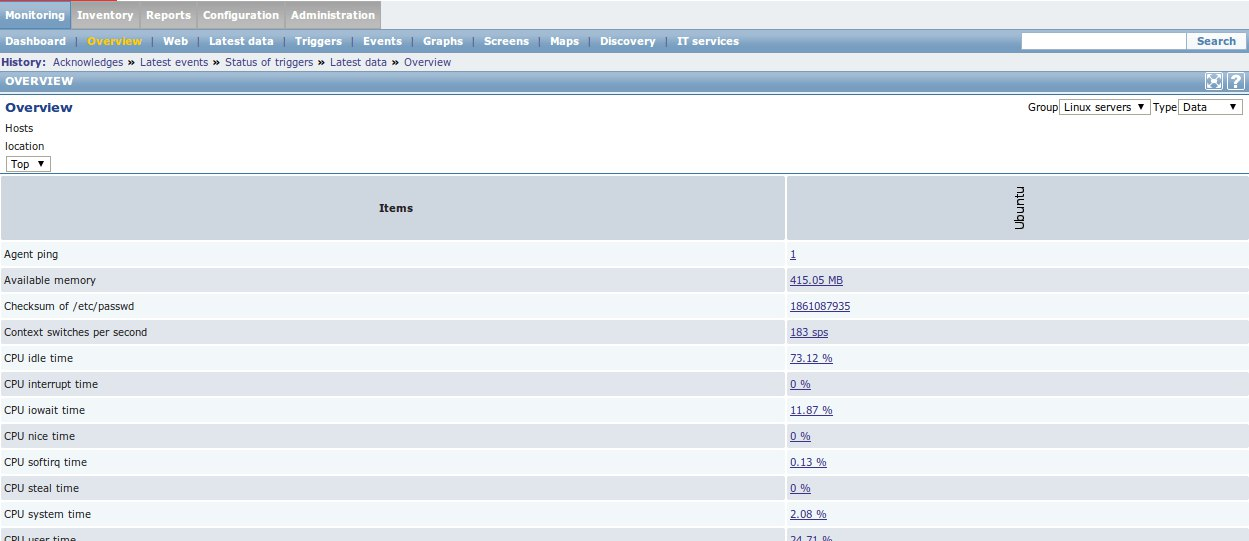
\includegraphics[width=0.8\linewidth]{eco/images/zbx.jpg}} 
\caption{Просмотр данных о сервере} 
\end{figure} 

Работа над шаблонами: 
\begin{itemize} 
\item Для начала были получены с устройств строки OID; 
\item Для каждой строки OID было написано правило обнаружения в шаблоне; 
\item Далее создавались элементы данных и триггеры; 
\item Были созданы несколько графиков. 

\begin{figure}[ht!] 
\center{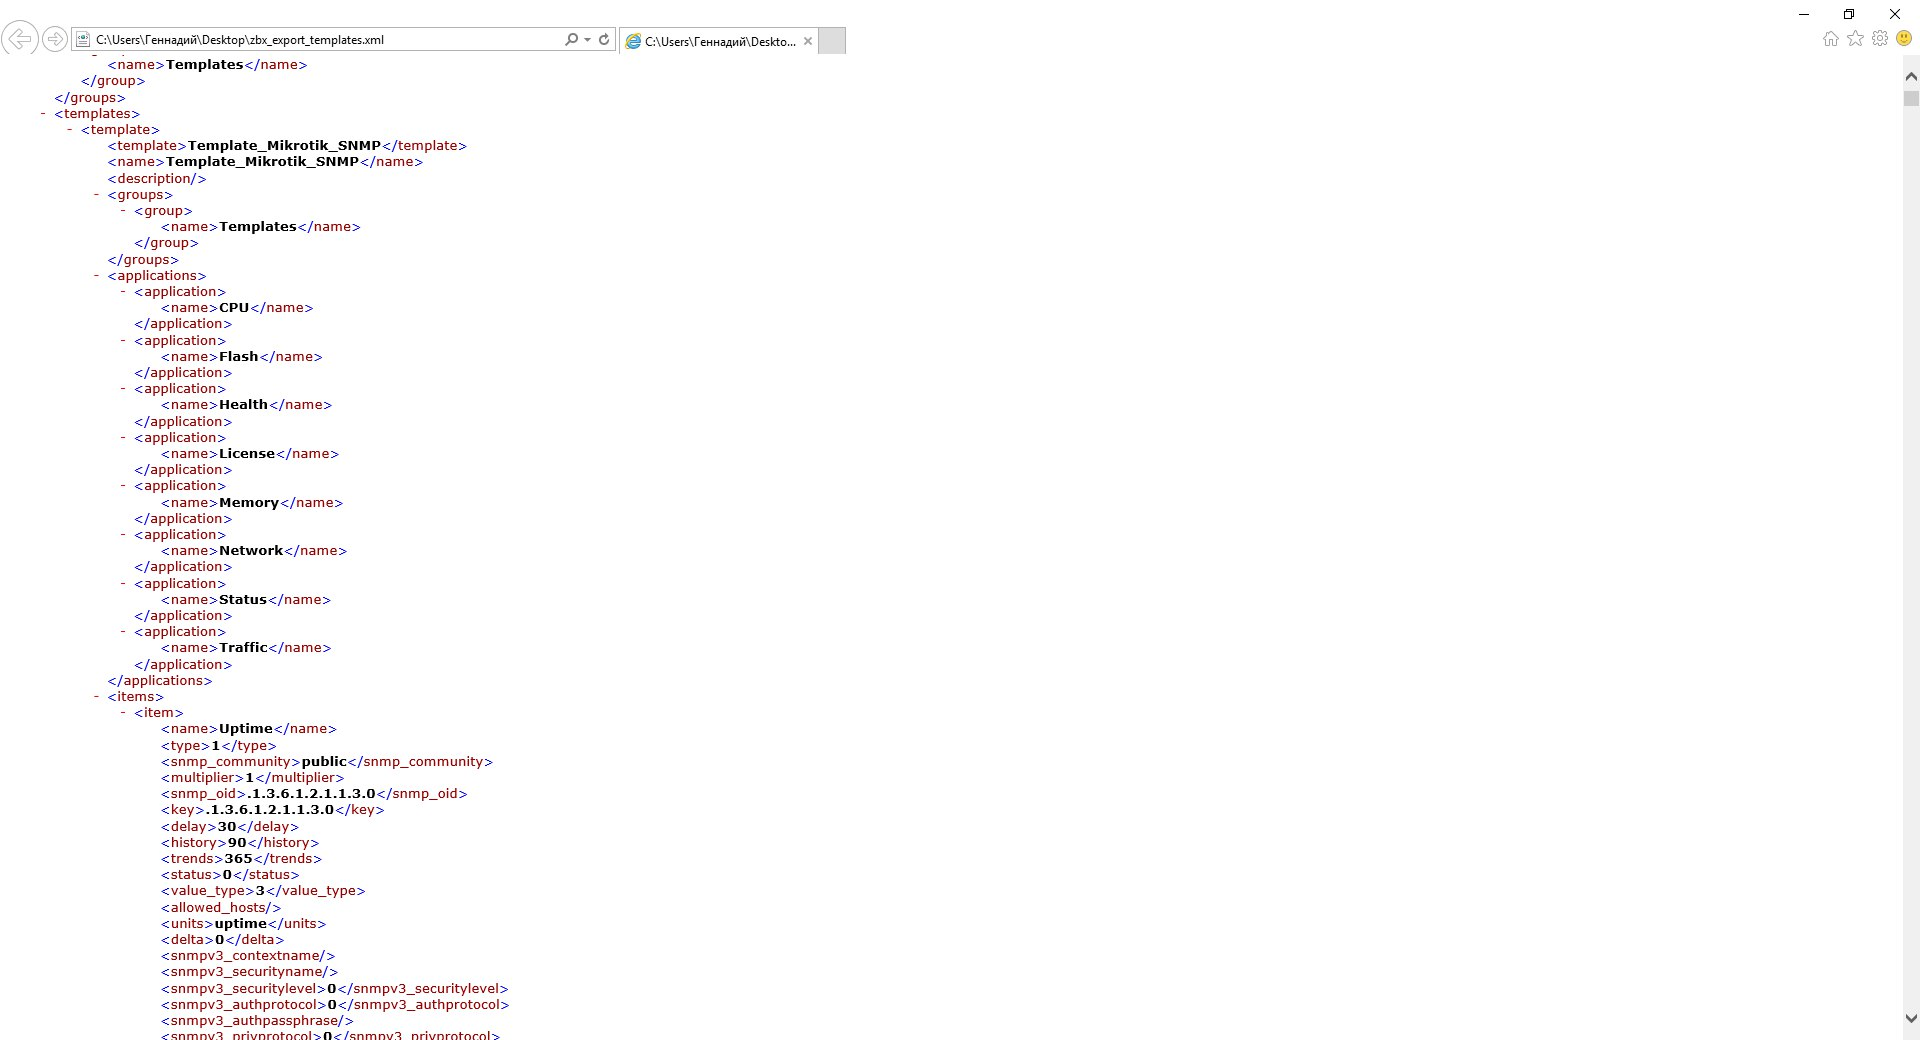
\includegraphics[width=0.8\linewidth]{eco/images/gena_zabbix.jpg}} 
\caption{Пример готового шаблона} 
\end{figure}